\documentclass[10pt,a4paper]{article}
\usepackage[utf8]{inputenc}
\usepackage{amsmath}
\usepackage{amsfonts}
\usepackage{amssymb}
\usepackage{a4wide} %Wider margins
\usepackage[english]{babel} %English dictionary for hyphenation and definitions, e.g. Table vs. Tabel
\usepackage[official]{eurosym} %Support for Euro-sign
\usepackage[utf8]{inputenc} %Support for internationalization, e.g. é vs.\’e
\usepackage{amsmath,amssymb,amsthm} %Support for mathematical formulas and symbols
\usepackage{fancyhdr} %Fancy headers
\usepackage{hyperref} %Creates clickable links
\usepackage{graphicx} %Support for grahpics
\usepackage{nopageno} %Support for removal of pagenumbers
\usepackage{tabularx}
\usepackage{enumitem}
\usepackage{xspace}
\usepackage{algorithm,algpseudocode}
\usepackage{float}
\usepackage{mathtools}
\usepackage[dvipsnames]{xcolor}
\usepackage[titletoc,toc,title]{appendix}
\usepackage{listings}
\usepackage{pdfpages}
\usepackage{footmisc}
\usepackage{attachfile2}
\graphicspath{ {./ThesisFigures/} }

\hypersetup{
    pdftitle={}, %PDF-file will be given a proper title when viewed in a reader
    hidelinks %PDF-file will be given clickable, yet not visible links when viewed in a reader
}
\newcommand{\documenttitle}{A Computational Biology Framework}
\newcommand{\documentsubtitle}{Creating a platform for biomedical engineers to efficiently do their research}


\newcommand{\true}{{\sc True}\xspace}
\begin{document}
	
	\begin{titlepage}
		
		\center
		
		\vspace*{3cm}
		
		\textbf{\huge \documenttitle}
		
		\textit{\LARGE \documentsubtitle}
		
		\vspace*{2cm}
		
		\large
		\centering
		T.P.A.~\textsc{Beishuizen}~(0791613)\\
		Biomedical Engineering - Computational Biology\\
		Data Engineering - Information Systems\\
		Eindhoven, University of Technology\\
		Email: \texttt{t.p.a.beishuizen@student.tue.nl}
		
		\vfill
		
		\vspace*{1cm}
		
		\today
		
	\end{titlepage}
	
	\tableofcontents
	
	%\newpage
	
	\pagestyle{fancy}
	%Abbreviations used by fancyhdr:
	%E Even page
	%O Odd page
	%L Left field
	%C Center field
	%R Right field
	%H Header
	%F Footer
	\fancyhead{} % clear all header fields
	\fancyfoot{} % clear all footer fields
	\renewcommand{\headrulewidth}{0.4pt}
	\renewcommand{\footrulewidth}{0.4pt}
	
	\fancyhead[L]{\rightmark}
	\fancyfoot[C]{\thepage}
	\fancyhead[R]{T.P.A. Beishuizen}
	
	
	\clearpage
	
	\section{Introduction}
	\label{sec:Introduction}
	
	% Quick explanation for biomedical data
	Biomedical Engineers are known to extract useful information out of biomedical data. The biomedical data can come from many different sources: hospitals, universities and private companies, but also publicly available data.  Currently, a standard is missing to analyse those data sets efficiently. With the vast number of data sets that are available, such a standard in the form of a framework on data analysis would be valuable. This framework can be a basis for researchers to start with their data analysis preventing them from creating everything from scratch.
	
	% Layout graduation project
	First an extensive background on important topics for such a framework is discussed. Four different parts are explained why they are important for the creation of such a framework. These parts are: biomedical data (data used for analysis), data analysis goal (how does a goal influence the choice of analysis), data analysis tools (which ones are usable) and at last biomedical knowledge (what engineers of BME and third parties already know about data analysis). After the extensive background research, a research question is formulated with several sub-questions for each of the four parts and a hypothesis as an answer for each of the four questions.
	
	\section{Background}
	\label{sec:Background}
	
	% Biomedical engineering description.
	Biomedical engineering can be seen as a specific part of engineering with a wide variety of topics. These topics are theoretical, non-experimental undertakings, but also state-of-the-art applications. Combining all of these different parts in one definition is not a simple task\cite{bronzino2014biomedical}. For this project, the focus is mainly on research and development, also known as knowledge discovery\cite{bramer2007principles}.
	
	% Biomedical research summary
	When a biomedical engineer begin with a project usually only a data set and a research goal are known. To achieve that goal from the data set, four different aspects influence the project's course and development:
	
	\begin{enumerate}
		\item[] At first obviously the data itself is an influencer as the data restricts the project in several ways. Examples of such restrictions are multidimensionality, set size, data heterogeneity, missing feature values and population handling.
		\item[] A second well-known influencer is the main research goal. Since the biomedical engineer wants to achieve a certain goal, the approach outcome should match that goal for the research to be successful. Most goals are focused around either data mining, extracting relations from available data, or modelling, creating a model within data features.
		\item[] The steps to take from data to goal do not only need an approach, but also a tool to execute it. A third influencer therefore, is the availability of data analysis tools. The choice of a certain tool has a big impact on the project, as each one of them has its own advantages and disadvantages. The two well known tools are MATLAB and Python, however some engineers are using R, Java or C++ and there are still other possibilities.
		\item[] A last big influencer is biomedical knowledge. What experience the scientist already has with similar projects can greatly influence the choice of approach and framework. Knowledge of the supervisor and publicly known information on the research subject from books and articles also influences the approach, as already known outcomes do not have to be researched again.
	\end{enumerate}
	    
	% Process steps for biomedical research
	Previous research projects on data mining called for a model how to retrieve patterns from data collections. Frameworks have been proposed, usually with a number of steps\cite{CIOS20021}. These suggested frameworks do not specifically fit the complete biomedical world for being too broad\cite{fayyad1996knowledge} or being too specific.\cite{cios2000knowledge} A customized framework is very beneficiary. 
	
	\subsection{Biomedical Data}
	\label{subsec:BiomedicalData}
	
	% Introduction biomedical data
	A big aspect of choosing how to set up the data analysis is the data itself. The amount of data in the biomedical world is growing at an enormous rate, faster than biomedical engineers can analyse. Several additional challenges came up with this uncontrollable growth. These challenges are mainly focused around data volume, dimensionality, complexity, heterogeneity and quality\cite{chen2006medical, doi:10.1093/bib/bbx044}.
	
	% Volume challenge
	Scientists are tempted to collect abundant data, which makes data sets bigger than needed. Both in number of instances and features, data sets are harder to understand or analyse when more instances and features are available.\cite{chen2006medical} This volume problem usually is tackled by taking sub-populations of the complete set. Sub-sets can either be focused around a part of the population (gender, age, race) or taken at random to still represent all of it. Due to the efficiency of analysis techniques and the rise in computational speed of servers\cite{blythe2008rise}, volume on its own becomes less of an issue. Volume does however become an issue when combining it with heterogeneity and quality\cite{Turkay2014, Holzinger2014}.
	
	% Dimensionality challenge
	Not all data sets have a high number of instances that cause a big data volume. Sometimes there are relatively few instances, while the number of features is proportionally high\cite{dubitzky2007fundamentals}. Usually many of those features are not relevant enough for the research, however are still used for testing. Trying to remove features that are not important greatly helps finding relations between the others and create more knowledge about the research topic. Lowering the number of features also makes the data volume go down, making analysis easier. Mainly an optimal features set should be selected to obtain the best results\cite{PENG201015}.
	
	% Low data volume challenge
	Another way to approach a high number of features for a low number of samples is that the number of samples is too low. If data is gathered for only a couple of patients, results will hardly ever be consistent. Most analyses require more samples and give biased results because of that. There are two ways of dealing with this low number of samples, the first one being generating more samples\cite{dunbar2006spatial, devroye1986sample} and the second one using the samples highly efficient\cite{van2002gene, roff1989statistical}. Most likely a combination fo both gives the best results. 
	
	% Complexity challenge
	Biomedical data can also be very complex. Useful results may be present, however it is very hard to obtain it. Examples of complex data are images, several biomedical signals and temporal data. Details of the useful results that are present in images is for example very hard to detect, the temporal data can vary quite much over time and the biomedical signals can be hard to combine with static biomarkers.\cite{Yoo2012} This aspect benefits from exchanging knowledge with other research areas that specialize in mining of those complex data sets\cite{Turkay2014, bellazzi2011data}.
	
	% Heterogeneity challenge
	The biggest challenge comprises of aligning different data sets. No standard for data sets is available and therefore data sets differ greatly from each other. Data is weakly structured or even unstructured\cite{Holzinger2014} and variables are processed differently due to other protocols or the collectors' preference of representation\cite{Otasek2014}. Also the variety of data is hard to combine when sources are fundamentally different. When parts of the data qre images, another part is a table from the laboratory and a third part is textual remarks of the doctor, standardizing merging those three is much harder than merging three lab sets. Those merges are also very prone to errors, as imprecisions can be vastly different between those data sets. No tool works directly with these raw data sets and preprocessing almost definitely has to occur beforehand\cite{CIOS20021, Turkay2014}.
	
	% Quality challenge
	A last challenge is about data quality. The data is usually gathered by doctors and laboratory workers. Since the data is manually gathered by humans, the data has a relatively high error rate. The data can be quite noisy, values can be inconsistent, wrongly entered or even missing.\cite{CIOS20021} Not only human errors cause the data quality to drop, but the heterogeneity, as well. Two hospitals can have different protocols for the same treatment and sample different biomarkers for that protocol. Due to that difference, biomarkers can be missing for some of the entries. The time of data gathering is also a big factor as some biomarkers change greatly over time. The databases are usually also built for financial purposes and not for research, which can hurt the quality.\cite{Yoo2012}
	
	% Standardized database
	These challenges within the data are greatly discussed.\cite{bellazzi2011data} Many proposals to tackle them are made, however none is actually widely adopted, yet, as a global standard for databases. Also, with the uncontrolled growth in biomedical data, it will become hard to have such a standard recognised all over the world.\cite{Otasek2014, marenco2004qis, bichutskiy2006heterogeneous, sperzel1991biomedical, aubry1988design, Windridge2014}  
	
	\subsection{Research goal: Data Mining}
	\label{subsec:ResearchTarget}
	
	% Introduction data analysis goals
	A second important part is the research goal. Available data is analysed with a certain goal in mind. This goal differs greatly for multiple projects and of course heavily influences the data analysis approach. Two major aspects are present for data analysis, data mining and modelling. For this project, the focus is on data mining.
	
	% Data mining definition
	Data Mining gains multiple definitions over the years. The most adopted definition is the following: “Data mining is the analysis of (often large) observational data sets to find unsuspected relationships and to summarize the data in novel ways that are both understandable and useful to the data owner\cite{hand2001principles}." As this definition states, the main goal is to find new and useful insights and patterns through datasets, that can be used in further decisions or hypotheses\cite{chen2006medical, 7024124}. It is one of the links that brought data and knowledge together\cite{Yoo2012}. A data mining project follows a certain layout. (Figure \ref{fig:ResearchSteps}), which in the end leads to further knowledge that aids the medical world.\cite{bramer2007principles} 
	
	\begin{figure}
		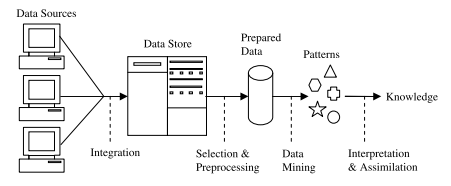
\includegraphics[scale=1.0]{ResearchSteps.png}
		\label{fig:ResearchSteps}
		\caption{A schematic overview how a project involving data mining is done. Multiple data sets are integrated in one database. Feature selection and preprocessing take place to prepare the data. Then the data is mined to find patterns. These patterns are then interpreted and assimilated to discover knowledge on the subject\cite{bramer2007principles}.}
	\end{figure}
	
	% Types of data mining
	Since biomedical data is a wide scope, data mining has several specialisations in different directions. An example will be text data mining, used to find related articles with websites such as Pubmed and Google Scholar. These articles can mention similar genes, diseases or proteins and give additional information about them. Another example is microarray data mining. This type of data mining focuses on extracting entities and pathways that define a disease or other phenotype. Two other data mining types are proposed. One focuses on extracting useful information out of mass spectrometry data points, called proteomic data mining. A second focuses more on a molecular level and how these molecules affect different cell types\cite{YANG2012S16}.
	
	% Reference to earlier made report
	Whichever splits are made in the data mining aspect for different areas in biomedical data analysis, the techniques are mostly based on statistical analysis and machine learning. A discussion of these two types have been made earlier report\footnote{\label{fn:BDA}Biomedical Data Analysis - \textit{Tim Beishuizen}}.
	
	\subsection{Data Mining Tools}
	\label{subsec:DataMiningTools}
	
	% Introduction data mining tools
	When applying several data mining algorithms to extract results from a data set, a certain tool has to be used that facilitated the use of those algorithms. Several basic tools are available and widely used\footref{fn:BDA}. Since biomedical data has specific characteristics, separate tools or frameworks consisting of those tools are made. These are usually made to create a database with a certain lay-out to put it in or to collect multiple algorithms and alter them specifically for biomedical cases. Many times both are connected as well, for optimized use.
	
	% Data set storage
	To store biomedical data several projects are started. Famous project examples are the Human Genome Project (HGP) that tries to sequence the entire human genome\cite{sawicki1993human} or the Human Connectome Project (HCP) that focuses on the brain connectivity\cite{van2012human}. Both consist of an enormous amount of data that needs to be stored and for both a tool is created for use in these project, for instance the ConnectomeDB for the HCP\cite{marcus2011informatics}. Similar projects resulted in biomedical databases, such as KEGG\cite{kanehisa2000kegg}, Reactome\cite{joshi2005reactome}, NCBI\cite{edgar2002gene}, GeneCards\cite{safran2010genecards} and HMDB\cite{wishart2007hmdb}. These databases store data about genes, metabolites and pathways and are used by numerous scientists to completely understand those. More databases are made or are in development, all of them for a specific domain in biomedical research.
	
	% Problems data frameworks and databases
	One immediate issue with all of theses existing databases is that hardly any framework or tool can be found for synchronisation of these databases. Some are available\cite{mork2001model, sujansky2001heterogeneous}, but their use is limited to a specific area only without any possibilities to switch in between. An all encompassing framework is not made. For that reason, multiple scientists make a tool specifically for their specific area. New scientists have a hard time using the newly created tool and try to create a new one themselves. To stop that cycle a new framework that combines aspects of the available tools will be very helpful\cite{teodoro2009biomedical}.
	
	% Biomedical data mining frameworks
	Several examples of tools and frameworks of biomedical data mining are available. A framework designed specifically for biomedical data was ImageJ\cite{schindelin2015imagej}. ImageJ can be used for biomedical image analysis and consists of image processing and analysis techniques. Another example is Genesis\cite{sturn2002genesis}, a platform for gene expression analysis based on Java and consisting of various preprocessing and clustering algorithms. Similarly the tools GeneCodis3\cite{tabas2012genecodis3}, FatiGO\cite{al2004fatigo} and \cite{zeeberg2003gominer} are created to interpret results from genomics generated data. Similar tools are made for metabolomics, such as Metscape 2\cite{karnovsky2011metscape} and MetaboAnalyst\cite{xia2015metaboanalyst}. A last example is the tool G*power3\cite{faul2007g} that focuses more on statistical analysis of biomedical data.
		
	\subsection{Biomedical Knowledge}
	
	% Introduction knowledge
	A last important aspect for data analysis is the available knowledge on the topic. Numerous scientists have done research on various biomedical topics. The knowledge gathered from these topics is available in several different ways\cite{bellazzi2011data}. Usually this information is found in a textual manner, in books, papers and articles describing the project results. Other information is found in the earlier mentioned databases, tools and designed algorithms. A third type of knowledge is implicit, scientists are expected to have certain skills, or should be trained for if not\cite{zupan2006knowledge}. All of these are interesting in their own ways.
	
	% Textual knowledge
	Literature knowledge is the basis for all research. The knowledge found on several different research areas can result in new insights and ideas for unexplored parts. The projects generated this way become knowledge-driven and have hypotheses based on gathered information\cite{bellazzi2011data}. Not only at the start of research projects knowledge is used, as it is a guide throughout the whole process. In the final project steps the results should be used to improve or extend the existing knowledge, so it can be used in new projects\cite{zupan2006knowledge}.
	
	% Data knowledge
	When looking at projects on implementation level, more interesting data knowledge can be gathered from databases, tools and algorithms. These three can be used to test and answer hypotheses derived from textual knowledge. Mainly these are used for data analysis as known data is gathered from databases, tools are used for their analysis properties and algorithms are implemented, all to improve the project results. When considering data mining and its tools (subsection \ref{subsec:ResearchTarget} and \ref{subsec:DataMiningTools}), everything known plays a big role\cite{bellazzi2011data}.
	
	% Scientist knowledge
	A third knowledge type is the implicit knowledge of the scientists conducting a research project. These scientist can have a big difference in background and therefore focus on different goals, tools or algorithms. Scientists should be familiar with using data mining tools to be able to use them, both in a general way as well as for specific tools. Frameworks are made with a certain type of scientist in mind as well, making it important that the desired type of scientist is able to use it\cite{zupan2006knowledge}.

	% Problems biomedical knowledge
	These types of knowledge can cause several issues. Projects will not be conducted properly if literature does not back up initial points of view and assumptions. On the other hand data knowledge that stems from other research projects can be used for continued improvement in the projects, that could not be done if this type of knowledge was not around. At problems could arise when scientists had different implicit knowledge. A physician at the hospital would not have the same knowledge as a professor in data mining, but would have a better understanding of the usefulness of the results. 
	
	\section{Research Question}
	\label{sec:ResearchQuestion}
	
	% Introduction research question
	The main goal is to create a framework for more efficient data analysis. Based around the four main influencers of data analysis, a main research question is made and divided in five separate sub-questions. The main question is:\\
	\\
	% Main question
	\emph{What aspects are of importance to include in a framework for Biomedical Engineers for more efficient data analysis?}\\
	\\
	As discussed earlier the main question could be divided in five different sub-questions. These five sub-questions would have their separate hypothesis. The five questions were:
	
	\begin{enumerate}

	% Data driven question
	\item[] \textit{Data driven:} How does the available data influence the choice for a certain data analysis approach?
	
	% Target driven question
	\item[] \textit{Target driven:} How does the research goal influence the choice for a certain data analysis approach?
	
	% Data mining tool driven question
	\item[] \textit{Tool availability driven:} Which available research tools should be included in this framework?
	
	% Data mining tool extension driven question
	\item[] \textit{Tool extension driven:} In which instances is extension required for completion of the framework?
	
	% Data knowledge driven question
	\item[] \textit{Knowledge driven:} How must both availability- and lack of knowledge be included in the framework?
	
	\end{enumerate}
	
	\subsection{Hypotheses}
	\label{subsec:Hypotheses}
	
	% Introduction
	Since there are five different sub-questions, also five hypotheses are formed. These hypotheses define the layout of the framework.
	
	\begin{enumerate}
		
		% Data driven question
		\item[] \textit{Data driven:} The available data mainly influences the choice for a certain data analysis approach when preprocessing. Several preprocessing actions should usually be done before actual research is possible.
		
		% Target driven question
		\item[] \textit{Target driven:} The research goal is mainly important for the data mining part of the project. This means that multiple steps of data mining are taken in an increasing zoomed in level to eventually achieve the final goal.
		
		% Data mining tool driven question
		\item[] \textit{Tool availability driven:} Three tools were chosen to be good additions to the framework: SciPy, scikit-learn and TPOT.
		
		% Data mining tool extension driven question
		\item[] \textit{Tool extension driven:} Three main extensions are thought to be beneficial for the framework: a global analysis tool, an extension for TPOT on a preprocessing level and a database integration tool.
		
		% Data knowledge driven question
		\item[] \textit{Knowledge driven:} As biomedical engineers are the main target fo the group, the framework will be directed mainly to them, with additions such as a GUI and useable data sets as examples for how to use the framework.
		
	\end{enumerate}
	
	\section{Implementation Approach}
	\label{sec:Approach}
	
	% Introduction
	The framework will be created with at the base these five questions. For each question a different approach is given how to handle that in the framework. For illustration of the framework a tree is created (Figure \ref{fig:FrameworkTree}) With help of this tree every approach is shown within the complete framework.
	
	\begin{figure}
		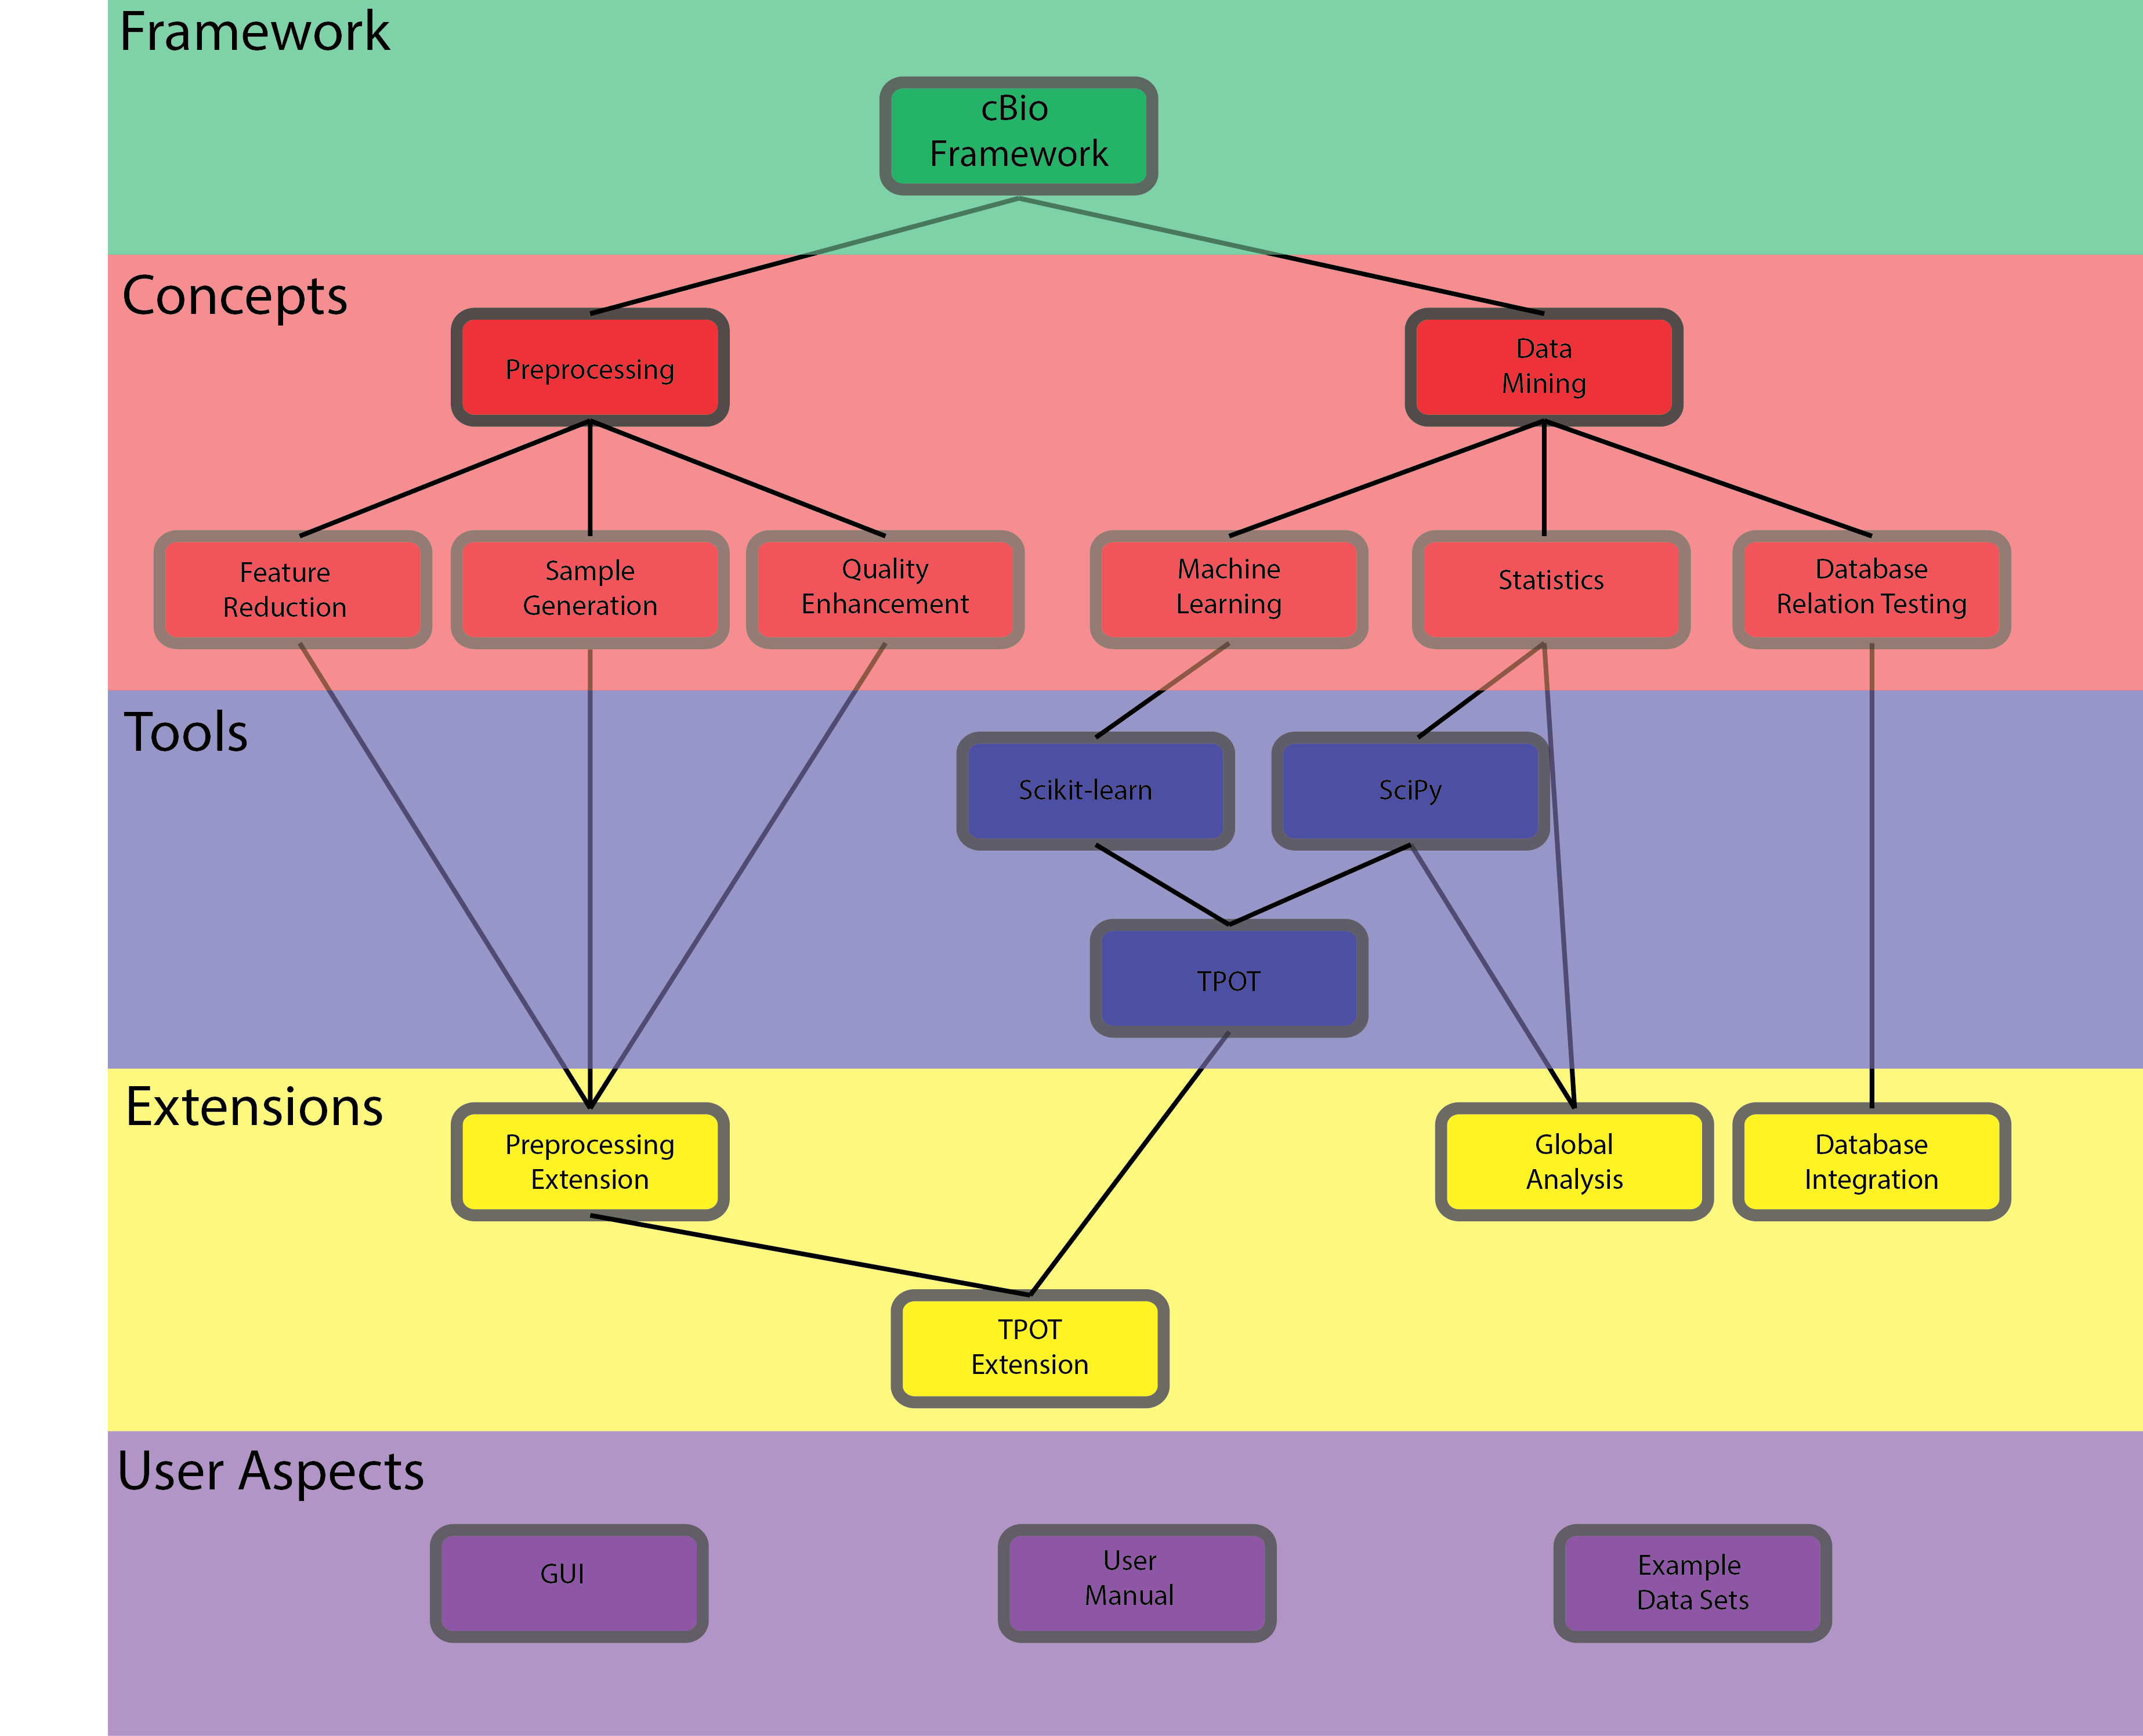
\includegraphics[width=\textwidth]{FrameworkScheme5i5.png}
		\caption{A schematic overview of how the framework eventually should look like. Every colour implied a different layer of implementation and corresponds to different approaches: (red) data driven and target driven, (blue) tool availability driven, (yellow) extension driven and (purple) knowledge driven.}
		\label{fig:FrameworkTree}
	\end{figure}
	
	\subsection{Data Driven Approach}
	\label{subsec:DataDrivenApproach}

	% Data challenges hypotheses
	A major part in a data driven analysis approach is the presence of challenges with preprocessing the data. Data volume, dimensionality, complexity, heterogeneity and quality challenges all are issues to be tackled, some of them more interesting than others. The most approachable three challenges are the data volume, dimensionality and quality challenges. These three problems were well known defined problems with various ways to deal with them, however no perfect answer existed yet. Data dimensionality can be tackled by various feature selection and reduction algorithms, such as principal component analysis, significance testing and clustering. Low data volume can be tackled by various data generation algorithms based on nearest neighbours and interpolation. At last data quality can be improved by handling for example missing values with interpolation and outliers with outlier detection. These three preprocessing aspects all are separately addressed in the framework at the concepts section (Figure \ref{fig:FrameworkTree}).
	
	\subsection{Target Driven Approach}
	\label{subsec:TargetDrivenApproach}
	
	% Target driven hypothesis, step one
	To reach a certain goal, several steps have to be taken. While the steps usually are vastly different, it always starts with a global analysis to localize possible issues and interesting features in the data. A statistical analysis is very beneficial for doing such a global analysis. Adding an easy possibility for such a global analysis would benefit the user.
	
	% Several algorithms for the goal
	Other steps are less clear. Follow-up steps after a global data analysis are trying out several basic techniques known to achieve that goal. After computing the results, they can be used to revise the technique for better results or disregarded completely. This more specific data mining step can be included trying out several machine learning techniques or better feature selection.
	
	% Specific algorithms for the goal
	The final steps to achieve the goal is very personalized for every project. To approach these final steps earlier results are used to obtain a final idea. This means that the scientist itself has the best idea how to achieve that goal with the knowledge gathered from the first couple of steps. Therefore it is not useful to guide someone in this part of the data analysis and no special focus is needed for this step.
	
	% Explanation of figure
	A small summary: he global analysis and basic techniques are part of data mining. Three parts are addressed for data mining: machine learning, statistics and database relation testing. These three data mining aspects all are separately addressed in the framework at the concepts section (Figure \ref{fig:FrameworkTree}).
		
	\subsection{Tool Availability Approach}
	\label{subsec:ToolAvailabilityDrivenApproach}
	
	% Introduction tool availability Python, scipy, scikit-learn, TPOT
	Tools to be included in the final framework must be focused around the data driven and target driven desired techniques. This means that it should include tools for feature reduction and selection, sample generation, missing value and outlier handling, global analysis and machine learning. On top of that the tools should be able to communicate easily, as they might be used in sequence.
	
	% Scikit-learn, TPOT
	The package scikit-learn from python provides already several algorithms for this problem and may be a good start for the framework. Several feature selection and machine learning algorithms are present and easily useable. A very welcome addition to scikit-learn is the Tree-based Pipeline Optimization Tool (TPOT) that automatedfinding the best machine learning algorithm with the best hyperparameters. TPOT uses both algorithms from scikit-learn and algorithms made by the user. These two are good tools for a successful data mining project.
	
	% Scipy, Python, Anaconda
	Both scikit-learn and TPOT are packages for Python. Another Python package that is helpful for the project is the SciPy package. SciPy is very useful for statistical analysis, due to the broad level of available statistical algorithms in it. Those algorithms can be used for global analysis and outlier detection as well as possible feature reduction. Anaconda is a Python distribution that could help you automatically download multiple packages, among others scikit-learn, SciPy and the widely used NumPy. This Anaconda is therefore a welcome addition, too.
	
	% Explanation of figure
	To summarize, the three tools that will be a big part of the framework are scikit-learn, SciPy and TPOT. These three are addressed at the tools section (Figure \ref{fig:FrameworkTree}).
	
	\subsection{Tool Extension Approach}
	\label{subsec:ToolExtensionDrivenApproach}
	
	% Initroduction tool extension
	With the mention of Scikit-learn, TPOT and SciPy, most aspects desired in the framework are at least partly covered. These three are not perfect for every data set though and might need more programming to better suit the framework. Also several data driven preprocessing algorithms to TPOT is needed to TPOT more suitable for biomedical data. 
	
	% Volume generation & missing value handling
	With the mentioned tools a good base for most of the desired parts in the framework are mentioned. The missing aspects that are not discussed, yet, would be the three types of preprocessing. These three and possible more algorithms for the other aspects can be programmed to show more variety in preprocessing and data mining. Methods that are created for these extensions are then also to TPOT, for more automated preprocessing.
	
	% Initial statistical analysis tool
	Some statistical methods are available for analysis in SciPy. These statistical methods must be called separate from each other in SciPy and no selection is made for an initial global analysis. Therefore a new method for doing that global analysis can be made, that borrows methods from SciPy to give the use insight in the dataset. This means it needs basic statistical methods, such as descriptive statistics computation, significance testing and multicollinearity testing. 
	
	% Database integration
	At last numerous online databases are available with both genomic and metabolic data in them, such as NCBI and KEGG. Some people make some possible integration packages for these databases, however these are not widely known or used. A possible tool extension for the framework is a possibility to download specific parts of these databases that contain useful information, so these can be used for further investigation of the genomic or metabolic data.
	
	% Explanation of figure
	The four different extensions are: preprocessing extension, TPOT extension, global analysis and database integration. All four are added to the framework at the extension section (Figure \ref{fig:FrameworkTree}).
	
	\subsection{Knowledge Driven Approach}
	\label{subsec:KnowledgeDrivenApproach}
	
	% Created for biomedical engineering students
	The framework is created for Biomedical Engineers. As Biomedical Engineers, the Computational Biology group of the Biomedical Engineering Department of the University of Technology Eindhoven are taken as a reference group. Since this group mainly consists of either experienced employees that are already doing a research projects or less experienced students, the best focus for this framework is biomedical students. They benefit the most from such a framework that can help them at the start of their projects. The scope of the framework is then people that have some minor programming skills and need guidance for better understanding and efficiency.
	
	% Create a GUI
	Since inexperienced programmers do not know immediately how to program in possibly a different language, a graphical user interface (GUI) is helpful, as well. This GUI can mainly help in the global analysis, but maybe also in running some initial calculations with TPOT. When using this GUI, programming is less important as a skill and therefore people do not need to figure out how the framework is designed. For programmers that need to use more specific methods, it still is possible to use it as packages for their own projects.
	
	% Create a user manual with also examples how to use everything
	To understand everything without too much difficulty a user manual will be made. This user manual will include (publicly available) data sets and show how the framework can be used exemplary with these data sets. This manual will make the framework more accessible for both inexperienced and experienced programmers and help them understand it quicker.
	
	% Explanation of figure
	The GUI, user manual and exemplary data set handling are the three ways to approach the knowledge driven aspects. These three are added to the framework at the Usability section (Figure \ref{fig:FrameworkTree}).
	
	\bibliography{../References/Citings} 
	\bibliographystyle{ieeetr}
	
	\appendix
	
\end{document}
